\chapter[Обзор]{Обзор прибора}
\label{chap:instrument_overview}

\begin{figure}%[]
  \centering
  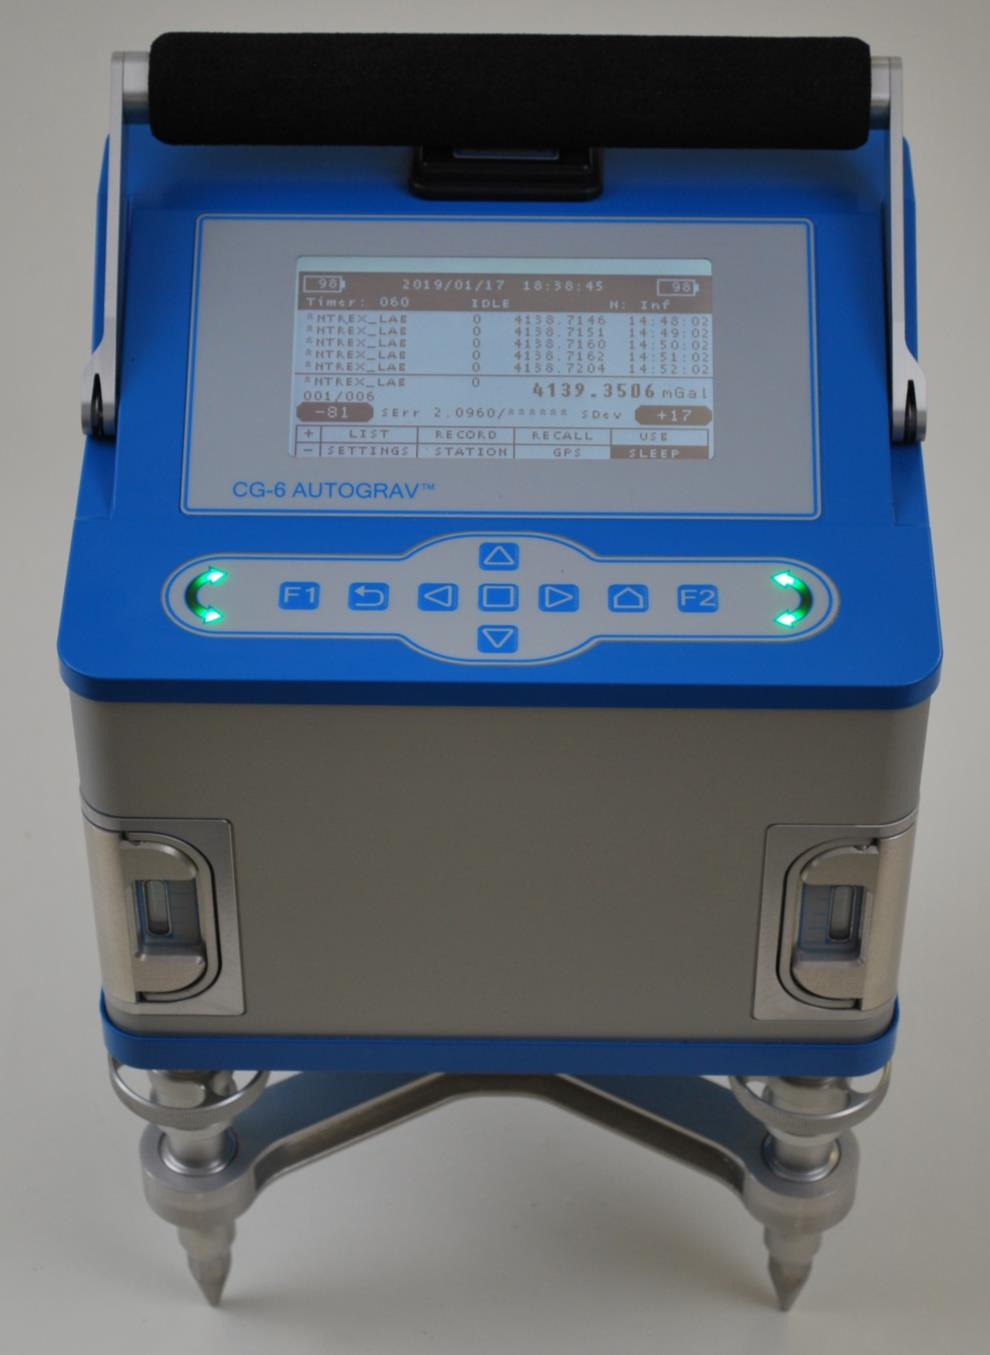
\includegraphics[width=0.9\textwidth, height=0.9\textheight, keepaspectratio]
  {figures/cg6_autograv}
  \caption{Гравиметр \cg{}}
  \label{fig:cg6_autograv_gravity_meter}
\end{figure}

\cg{}~-- это автоматический гравиметр, способный выполнять
измерения в любой точке мира с разрешением 0,0001 мГал в диапазоне 8 000
мГал. Прибор позволяет проводить как детальные микро гравиметрические
измерения, так и крупномасштабные региональные геодезические исследования.

Измерение выполняется простым нажатием клавиши, и в большинстве случаев процесс
измерения занимает менее одной минуты. Предусмотрена возможность выбора
дополнительных информационных циклов. \cg{} выполняет измерения,
обрабатывая непрерывную последовательность отсчётов длительностью 0,1 секунда.
Измерение вместе с выбранными внесёнными поправками отображается на ЖК-дисплее
непосредственно в мГал. Полученные данные сохраняются в памяти прибора, откуда
можно произвести их экспорт в любое удобное время.

Гравитационный датчик, электронные схемы и аккумуляторные батареи размещаются
внутри корпуса прибора.

Для защиты от изменений внешней температуры и атмосферного давления
чувствительные элементы \cg{} помещены в герметичную
термостабилизированную камеру. Благодаря широкому диапазону рабочих
температур~-- от \textminus{}40\textcelsius{} до +45\textcelsius{}~-- систему
\cg{} можно использовать в самых разных условиях окружающей
среды. Предлагается также версия прибора для высокотемпературных районов с
диапазоном рабочих температур от \textminus{}40\textcelsius{} до
+55\textcelsius{}.

Встроенные датчики наклона предоставляют системе \cg{}
информацию об угле наклона~-- это позволяет в режиме реального времени вводить
поправки в результаты измерений, выполняемых на неустойчивом грунте.

Горизонтирование прибора \cg{} не представляет сложности,
благодаря наличию двух стрелок со светодиодной подсветкой на панели прибора. Эти
стрелки показывают оператору направление, в котором нужно вращать винты треноги.

Две встроенные перезаряжаемые Li-ионные аккумуляторные батареи обеспечивают
систему \cg{} достаточной энергией питания для работы в
течение стандартного дня съёмки.

Внешний планшетный компьютер позволяет оператору легко настраивать рабочие
параметры системы \cg{} и сохранять эти настройки, а также
планировать и сохранять пункты съёмки. Планшетный компьютер поставляется с
установленным программным обеспечением LynxLG Land Gravity, с помощью
которого оператор может планировать предстоящую съёмку, осуществлять
удалённые измерения и непрерывный мониторинг сигналов силы тяжести и угла
наклона. Помимо прочих разнообразных функций планшетного компьютера, можно
отметить доступ к картам.

Если эксплуатация системы осуществляется при температуре окружающей среды ниже
\textminus{}20\textcelsius{}, рекомендуется использовать комплект
принадлежностей (номер 888405) для холодной погоды.

Среди других имеющихся принадлежностей~-- рюкзак Seco (\textnumero{}~140220) и тренога
для измерения градиента (No 101370004).
